\documentclass{article}
\usepackage{graphicx}
\title{Information visualization}
\author{Ari Viitala}
\begin{document}
	\maketitle

\section*{Exercise 1}
Yes.
\section*{Exercise 2}

\section*{Exercise 3}

The phenomenon where the gray line on darker background looks lighter than the one on the lighter background can be explained by how the human eyes ganglion cells that receive the light impulse are organized. The cell consists of an inner circle that sends more pulses as it receives light and an outer circle that send less pulses when it receives light. This means that the light received by the outer circle inhibits the light received by the inner circle.

Now when there is a steep gradient in the shade of color, the inner and outer circles receive different amounts of light. For example in the case of the darker background when he inner circle cells receive impulse from the gray area and the outer cells receive impulse from the darker area the outer cells inhibit signals sent by the inner cells less. This means that the gray appears lighter. The effect is reversed in the light background case where outer cells receive more light and thus inhibit the signal more making the gray appear darker.

The Difference of Gaussians model must be kept in mind when designing color scales because it alters how humans perceive changes in the lightness of colors. This means that the absolute value of the color in scale is not the only thing that contributes to how the information is perceived. Also the intensity of the shades around it affect the value communicated.  

\section*{Exercise 4}

White balance setting is needed because the distribution of light is different based on the light source. Outdoors the light from the Sun contains more blue photons than light from for example light bulb or a fluorescent lamp. Human brain and eye can adjust to different amounts and distributions of photons. This can be seen in for example the night mode filters for computer screens which filter out blue light. At first when the filter is applied the image color balance looks weir but after a while the image starts to look normal as the brain adjusts to the new type of light.

The digital camera sensor is different to the human eye as it just counts the amount certain energy of photons hitting it. If all images were saved as raw images with just the counts and energies of the photons everything would be fine as the color balances could be adjusted such that it looks right to the human eye. 

Raw images, however, require a lot of space and that is why normally digital images are compressed. In this compression comes the problem since the compression algorithm needs to interpret the raw data such that it matches how the human brain would  interpret that photon distribution. For example outdoors blue light would have to be suppressed in order to correct the image and outdoor mode does exactly this. This is why if we use the outdoor mode indoors the blue light is over suppressed and the image becomes red. Vice versa, if indoor mode is used outside, blue light is no suppressed enough and the photo ends up being blue.

\section*{Exercise 5}  

In figure \ref{glyphs} is presented the asked glyph. The glyph can represent four variables with it's size, shape, color and the deepness of the color. Out of these the size of the glyph and the deepness of the color can be continuous if desired. Shape and color are discrete and they can be extended outside the set presented here. 

I think all of the variables are pretty easy to distinguish but if the glyph size gets small then maybe round and hexagonal glyphs can become a bit difficult to distinguish. Also the darker colors can be harder to distinguish in the extremes they are all more or less black or white when we get to really dark or light shades.
\begin{figure}[h!]
	\centering
	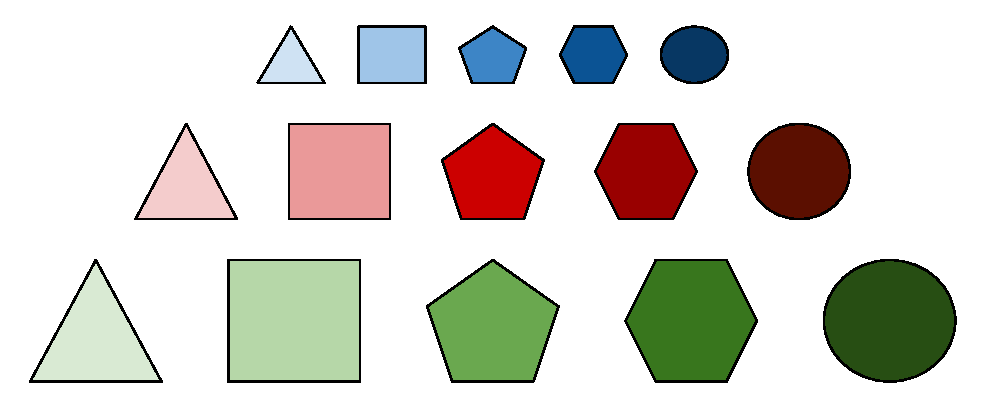
\includegraphics[width = \linewidth]{glyphs}
	\caption{A glyph set that is capable of representing four variables}
	\label{glyphs}
\end{figure}

\end{document}